\documentclass[10pt]{beamer}

\mode<presentation>
{
  \usetheme[height=1.25cm]{Madrid}
  \setbeamertemplate{navigation symbols}{}
  \setbeamercolor{alerted text}{fg=illini}
}
\usebackgroundtemplate{
\includegraphics[width=\paperwidth,height=\paperheight]{uc-background}}

\usepackage[english]{babel}
\usepackage{epsfig,subfigure,bm}
\usepackage{multimedia}
\usepackage{psfrag}
\usepackage{animate}

%%%%%% Begin of my macros and options

\setbeamertemplate{section in toc shaded}[default][55]
\setbeamertemplate{subsection in toc shaded}[default][55]
\setbeamercolor{block title}{fg=white,bg=illini}
\setbeamercolor{block body}{fg=black,bg=mygrey}

\setbeamercolor{emphprimary}{fg=CBlue}
\setbeamercolor{emphsecondary}{fg=illini}
\setbeamercolor{emphtertiary}{fg=mygreen}
\definecolor{darkForestGreen}{rgb}{.1,1,.1}
\definecolor{veryLightGray}{rgb}{.9,.9,.9}
\definecolor{greenApple}{rgb}{.3,.9,.3}

\setbeamercolor{frametitle}{bg=CBlue}   
\setbeamercolor{title}{bg=CBlue}

\usepackage{amsmath,amssymb,amsxtra,amsthm}
\usepackage{algorithm,algorithmic}
\usepackage{natbib}
\usepackage{bibentry}
\usepackage{xspace}
\usepackage{changepage}

\pdfmapfile{+sansmathaccent.map}

\definecolor{myblue}{rgb}{.2,.2,.7}
\definecolor{myred}{rgb}{.7,.2,.2}
\definecolor{mygreen}{rgb}{.2,.7,.2}
\definecolor{mygrey}{rgb}{0.9,0.9,0.9}
\definecolor{CBlue}{cmyk}{1,0.25,0,0}
\definecolor{illini}{rgb}{0.98,0.4,0.05}
\definecolor{black}{cmyk}{0,0,0,1}

\newcommand{\myemph}[1]{{\usebeamercolor[fg]{emphprimary}
    \textbf{#1}}}
\newcommand{\myemphalt}[1]{{\usebeamercolor[fg]{emphsecondary}
    \textbf{#1}}}

\graphicspath{{figs/}}

\title[Math for Robotics] % (optional, use only with long paper titles)
{CSE276C - Polynomial Interpolation and Approximation}

\author[H.~I. Christensen] % (optional, use only with lots of authors)
{Henrik I.~Christensen}
% - Give the names in the same order as the appear in the paper.  -
% Use the \inst{?} command only if the authors have different
% affiliation.

\AtBeginSection[]
{
   \begin{frame}
       \frametitle{Outline}
       \tableofcontents[currentsection]
   \end{frame}
}

\institute[UCSD] % (optional, but mostly needed)
{
  \begin{minipage}[c]{.2\textwidth}
    
\includegraphics[width=.65\linewidth]{ucsealnew}%
  \end{minipage}%
  \begin{minipage}[c]{.6\textwidth}
    \small
%%    \begin{center}
      Computer Science and Engineering\\
      University of California, San Diego\\
      \myemph{\url{http://cri.ucsd.edu}}\\          
%%    \end{center}

  \end{minipage}
%%  \vspace*{1ex}
}
%% - Use the \inst command only if there are several affiliations.
%% - Keep it simple, no one is interested in your street address.

\bigskip

\date[Oct 2020]% (optional, should be abbreviation of conference name)
{\small%
  October 2020}

\begin{document}
  
\nobibliography{/Users/hic/Dropbox/bibliography/bib-file}
\bibliographystyle{plain}


\begin{frame}[plain]
  \titlepage
\end{frame}


\section{Introduction}

\begin{frame}
  \frametitle{Introduction}
  \begin{itemize}
  \item Last time we spoke about direct use of data point / simple models
  \item What if we want an explicit functional approximation to data? 
  \item Approximating a function/data by a class of simpler functions
  \item Two main motivations
    \begin{enumerate}
    \item Decomposition of a complicated function into constituent simpler functions to simplify further work
    \item Recover a function from partial or noisy information
    \end{enumerate}
  \item Applications:
    \begin{enumerate}
    \item Signal compression / reconstruction (Fourier would be an example)
    \item Data fitting (line, plane, manifold, ...)
    \item Recovery of a model say CAD recovery
    \end{enumerate}
  \end{itemize}
\end{frame}

\begin{frame}
  \frametitle{Material}
  \begin{itemize}
  \item Numerical Recipes: Chapter 3.4-3.5
  \item Numerical Renaissance: Chapter 5
  \end{itemize}
\end{frame}

\section{Uniform approximation}

\begin{frame}
  \frametitle{Uniform approximation by polynomials}
  \begin{itemize}
  \item Looking at polynomial again
  \item What is the best uniform approximation? 
  \item Given a function f: $[a,b] \rightarrow R$ and a polynomial p we can measure the error by the $L_{\infty}$ norm, i.e.,
    \[
      ||f-p||_{\infty} = \max_{a<x<b} | f(x) - p(x) |
    \]
  \item A good approximation is one where the norm is small
  \item Remember Weierstrass' theorem. 
  \end{itemize}
\end{frame}

\begin{frame}
  \frametitle{Polynomial approximation}
  \begin{itemize}
  \item Lets restrict the degree of the polynomial - n
  \item Let set $\pi_n$ be all the polynomials degree at most n
  \item Let {\em uniform distance} of f from $\pi_n$ be the smallest
    error achievable using polynomials from $\pi_n$ denoted by
    \[
      d(f,\pi_n) = min_{p\in \pi_n} ||f - p ||_{\infty}
    \]
    
  \item How can we make it happen? 
  \end{itemize}
\end{frame}

\begin{frame}
  \frametitle{Polynominal approximation - getting help}
  \begin{itemize}
  \item We have a theorem:
    \begin{itemize}
    \item A function f continuous in $[a,b]$ has exactly one best
      solution from $\pi_n$
    \item The polynomial $p \in \pi_n$ of f across $[a,b]$ iff
    \item there are n+2 point $a \leq x_0 \leq \ldots \leq x_n+1 \leq b$ such that
      \[
        (-1)^i [ f(x_i) - p(x_i) ] = \epsilon ||f-p||_{\infty}
      \]
      where $\epsilon = signum[f(x_0)-p(x_0)]$ 
    \end{itemize}
  \item By alternating signs at n+2 points the different between f and p is precicely equal to the $L_{\infty}$
  \end{itemize}
\end{frame}

\begin{frame}
  \frametitle{Putting theorem to work}
  \begin{itemize}
  \item Can we use the theorem to build a strategy? 
  \item Lets consider $f(x) = e^x \mbox{ on } [-1, 1]$
  \item What would be the best 1st order approximation, i.e., $\pi_1$
    \centerline{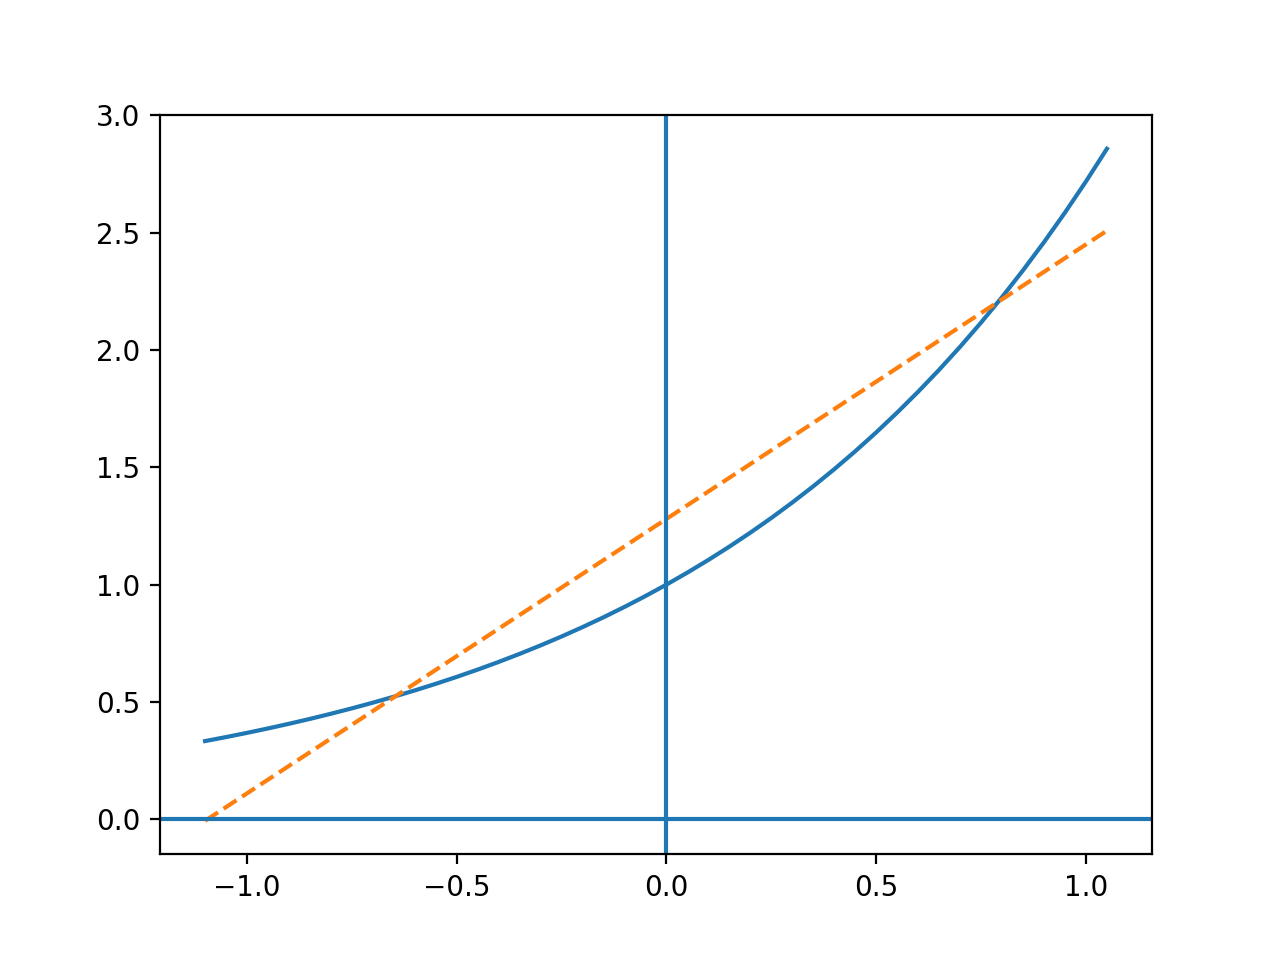
\includegraphics[height=5cm]{figure_1}}
  \end{itemize}
\end{frame}

\begin{frame}
  \frametitle{Fitting the line}
  \begin{itemize}
  \item So we have three points
  \item $x_0 = -1$, $x_1 = ? $ and $x_2 = 1$ 
  \item at which the error is $f(x) = p(x)$
  \item So what  is $x_1$?
  \item we can write $p(x) = a + b x$
  \item We can compute the error at the three points:
    \[
      \begin{array}{llll}
        e(x_0) & = f(x_0) - p(x_0) & = f(-1) - p(-1) & =\frac{1}{e} - a + b\\
        e(x_1) & f(x_1) - p(x_1) & = &  e^{x_1} - a + b x_1\\
        e(x_2) & f(x_2) - p(x_2) & f(1) - p(1) & e - a - b\\
      \end{array}
    \]
    
  \item Given $e(x_0) = e(x_2)$
    \[
      \begin{array}{ccc}
        \frac{1}{e} - a + b & = & e - a - b\\
        2 b & = & e - \frac{1}{e} \\
        b   & = & 1.1752\\
      \end{array}
    \] The slope must be equal to the average change
  \end{itemize}
\end{frame}

\begin{frame}
  \frametitle{Fitting the line (cont)}
  \begin{itemize}
  \item 
  \end{itemize}
\end{frame}

\section{Chebyshev Approximation}

\section{Trunkated Power Series}

\section{Summary}



\end{document}

%%% Local Variables:
%%% mode: latex
%%% TeX-master: t
%%% End:
